\documentclass{article}
\usepackage{graphicx} % Required for inserting images
\usepackage{amsmath}
\usepackage{float}  % Add this to your preamble
\usepackage{listings}
\usepackage{xcolor}

\title{ESD Individual Project}
\author{Andrew Trepagnier (alt658) }
\date{November 22, 2024}
\usepackage{float}  % Add this to your preamble
\usepackage{graphicx}  % For including graphics
\usepackage{amsmath}  % For align* environments

\begin{document}

\maketitle

\section{Introduction}

The purpose of this report is to provide the methodology and analysis for optimizing the flow rate of a piping water loop consisting of approximately 100 feet of 2" SCH. 40 pipe with 10 elbows, 6 gate valves, and two heat exchangers(finned tube cross flow with air mixed, water unmixed) in series.

Optimizing energy systems with computation simulations is critical to ensuring a system makes the most effective use of equipment life and energy. This water loop simulation was modeled in python. Below is a break down of key sections.
\begin{itemize}
    \item Mathematical Models
    \item System Head Loss Relationship
    \item Curve Fitting Manufacturer Data
    \item Validation of Equation
    \item Steady State Points
    \item Heat Exchanger Analysis
    \item Conclusion
\end{itemize}


The steady state point of the system will be dependent on the desired pump, motor, and impeller size. For this simulation, we will be analyzing the 0.5x3-7 Goulds Pump with a 6-in. rotor, pumped by a 3500 rpm motor.


\section{Mathematical Models}

After defining all of the known information about the piping network, including length, diameter, relative roughness, and more, the mathematical models are defined as functions of flow rate, Q [GPM]. This will enable the head loss to be plotted over an array of varying flow rates. 

\subsection{Each Function Used in Simulation}
Heat Exchanger Losses(Given):
$h_{x} = 0.0049Q^{1.852}$

Overall HT Coefficients(Given):
$U = \left(\frac{1}{13Q^{0.8}} + 0.047\right)^{-1}$

Reynold's Number(with gpm to $ft^{3}$ conversion):
$Re = \frac{4(\frac{1}{60})(\frac{0.134}{1})Q\rho}{\pi D_i\mu}$

Friction Factor- Turbulent:
$f = \frac{0.3086}{\left[\log_{10}\left(\frac{6.9}{Re} + \left(\frac{\epsilon}{3.7D_i}\right)^{1.11}\right)\right]^2}$

Friction Factor - Laminar:
$f = \frac{64}{Re}$

Total Minor Loss Coefficient(Given):
$K_{total} = 6(8f_t) + 10(30f_t)$

Major Loss:
$h_{f,minor} = K_{total}\frac{\left(Q\frac{1}{60}\frac{0.134}{1}\right)^2}{2g_cA^2}$

Total Head Loss:
$ h_{total} = h_{f,minor} + h_{f,major} + 2h_x $

\section{System Head Loss}

\begin{figure}[!ht]  % Added !ht for stricter placement
    \centering
    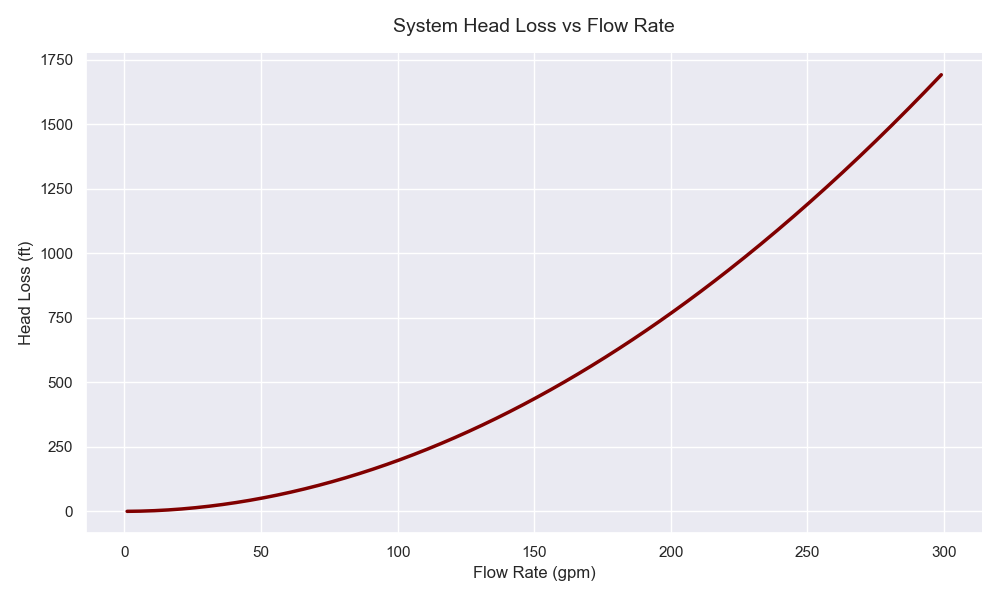
\includegraphics[width=0.75\linewidth]{sns_system_headloss.png}
    \caption{System Head Loss Relationship}
    \label{fig:enter-label}
\end{figure}

Plotting total head loss over a range of flow rates will give the system's relationship to total head loss. Frictional losses in the piping wall, fittings, and heat exchangers contribute to the total head losses in the system.


\section{Curve Fitting Manufacturer Data}
Separately, we can extract data from Gould's 0.5x3-7 Pump Curve at the 6", 6.5", and 7" impeller sizes. For this project, we are seeking the steady state point for a 6" impeller; however, the 6.5" and 7" impellers where plotted as well to illustrate how impeller sizes create varying steady state points.

\subsection{Curve Fitting Manufacturer Data}
In this analysis, five data points were extracted from the manufacturer data sheet. By utilizing a python library, Scipy. Fitting procedures can be easily called and modeled to any nth-order polynomial users would like. For this simulation, a quadratic fit the data perfectly. The 6" impeller's fitted equation intersected with the system head loss relation at [84, 138]. This tells us that for a Gould's 0.5x3-7 pump with a 6" impeller, the system is optimal at a flow rate of ~84 GPM and can supply the system with 138 feet of head.

\begin{figure}[H]
    \centering
    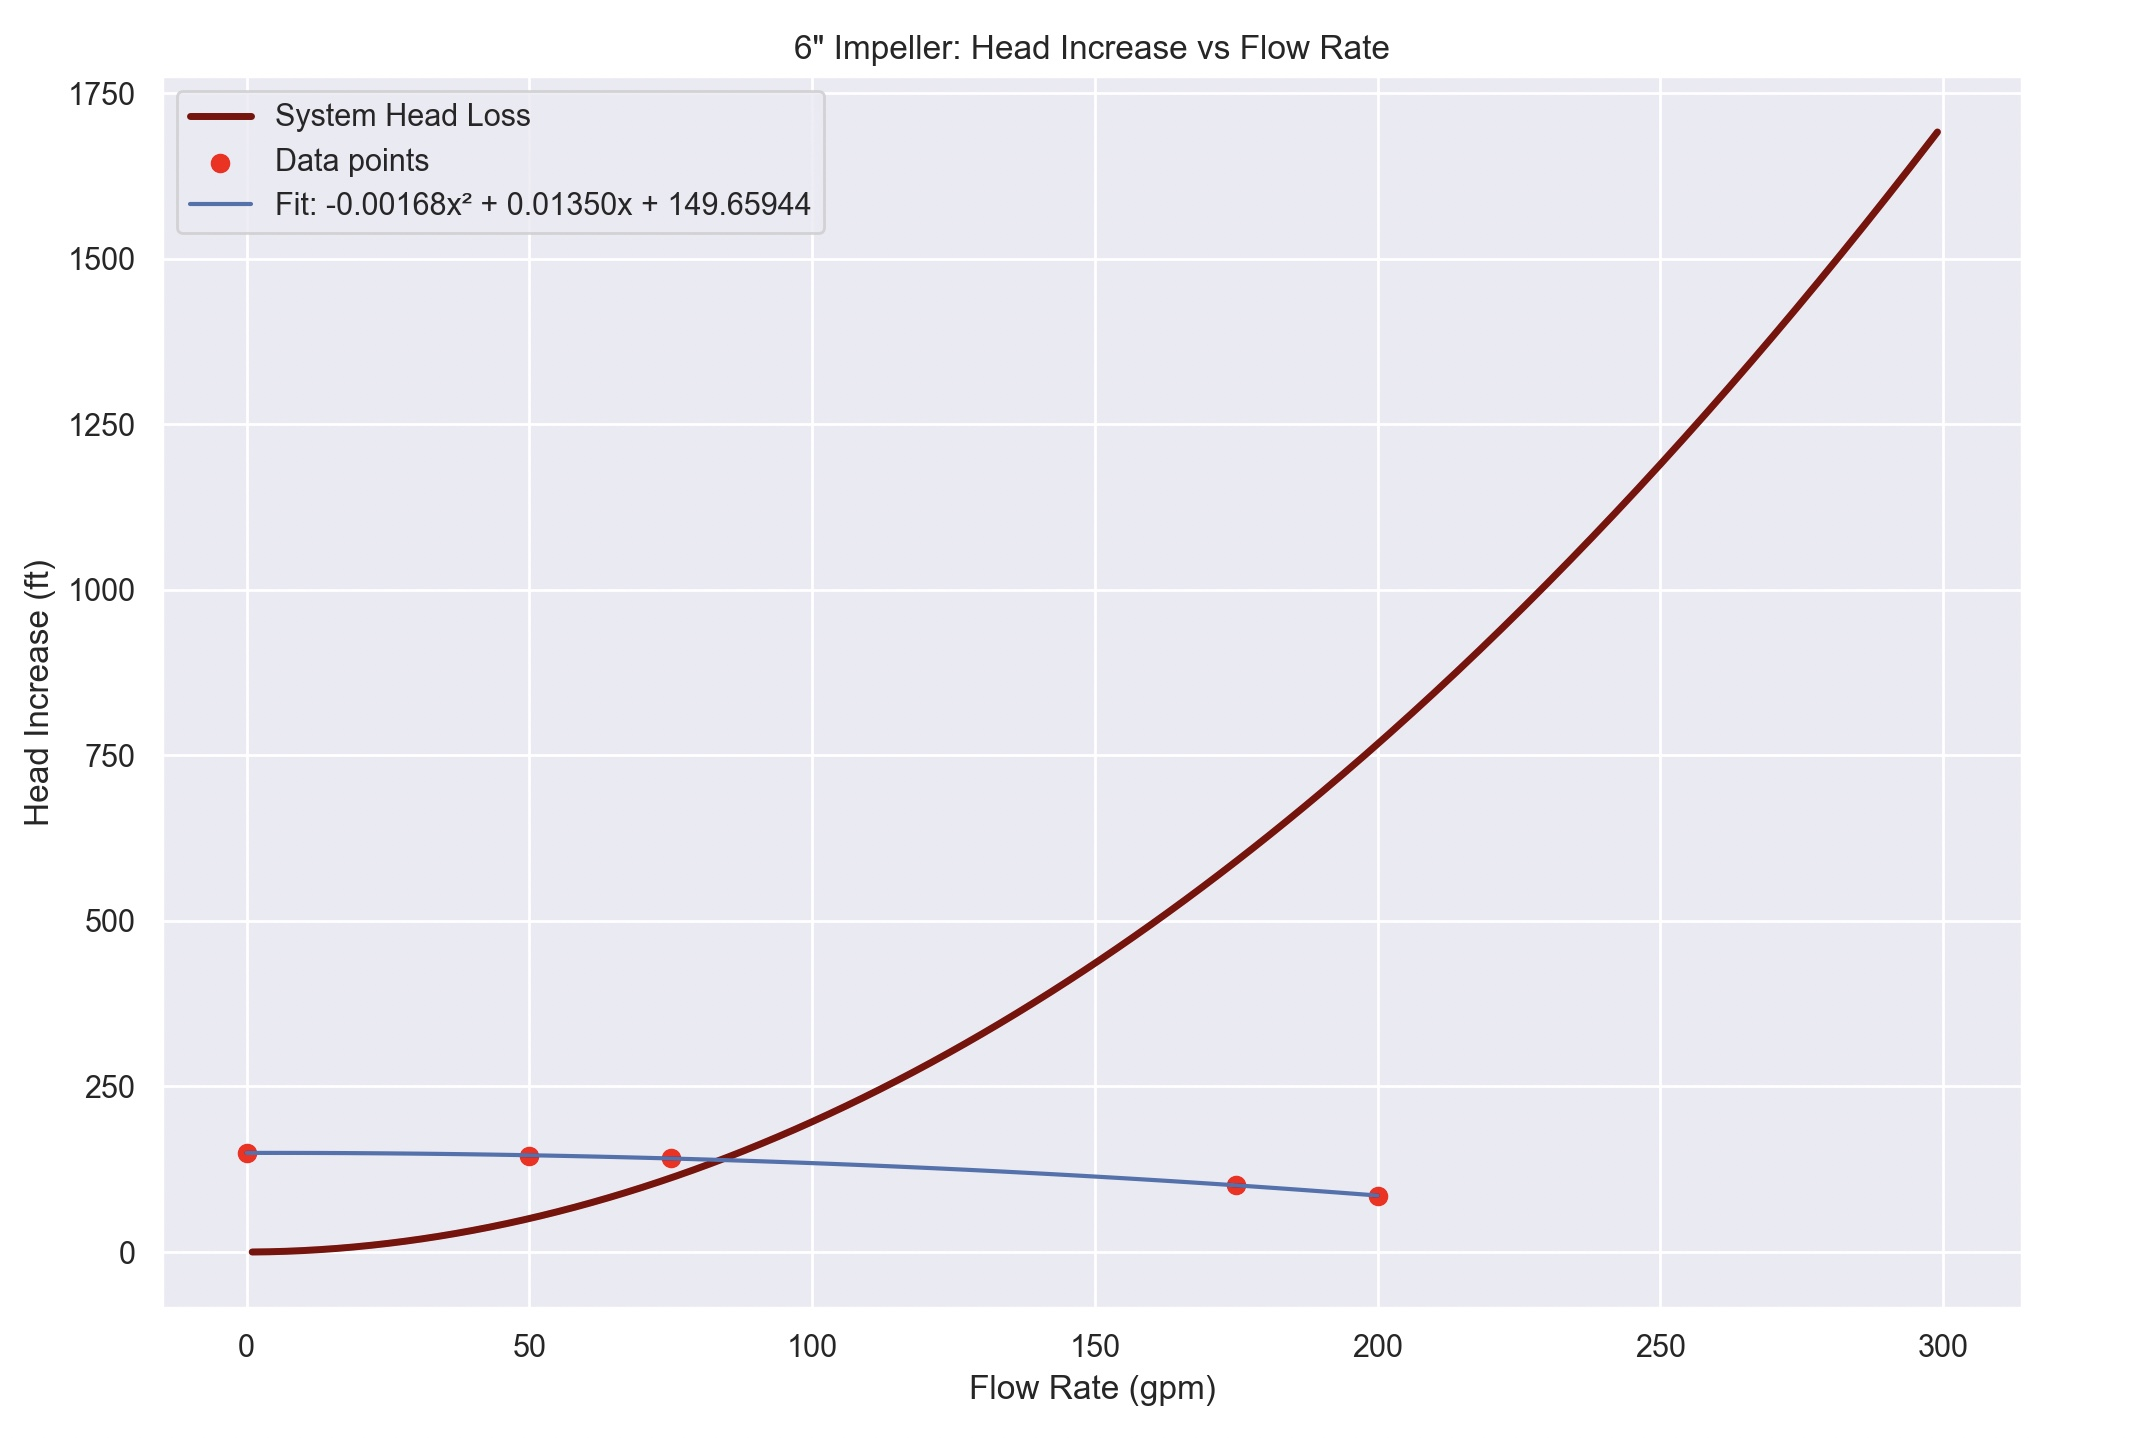
\includegraphics[width=0.75\linewidth]{AE5D4372-A838-4EA3-B71D-1255726D846A.jpeg}
    \caption{Steady State Conditions for 6" Impeller}
    \label{fig:impeller_6}
\end{figure}

\begin{figure}[H]
    \centering
    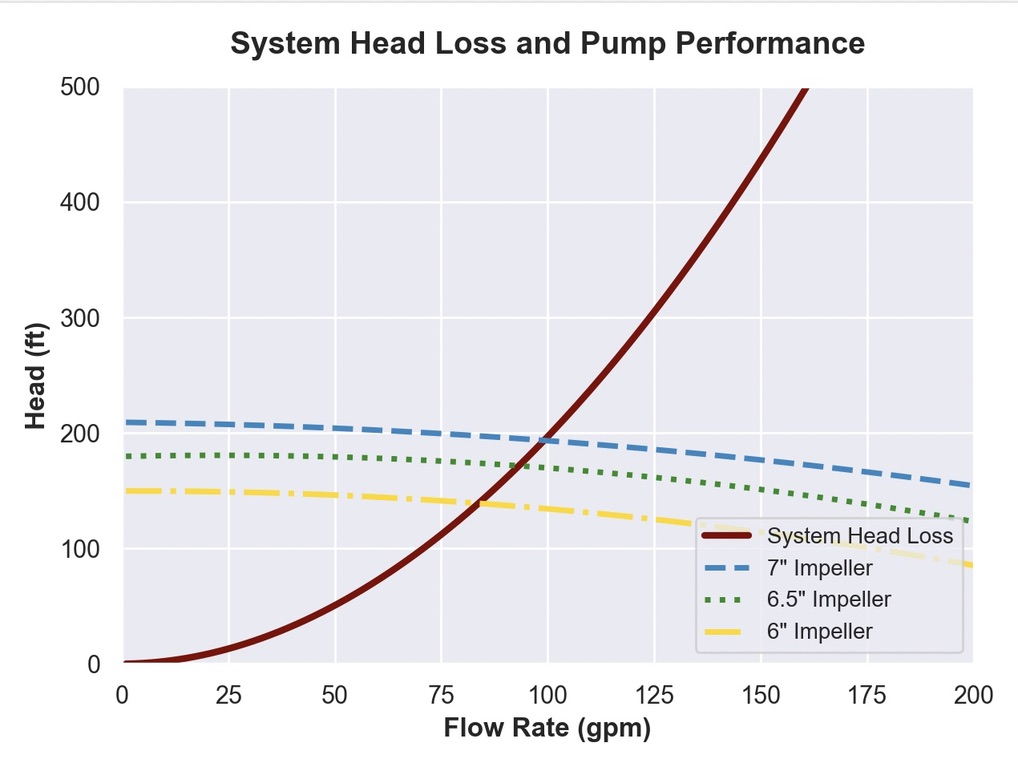
\includegraphics[width=0.75\linewidth]{95E131CE-68DB-4A4F-AEBB-CE40D397E913_1_105_c.jpeg}
    \caption{Steady State Conditions for Various Impeller Sizes}
    \label{fig:vary_impeller}
\end{figure}


\section{Heat Transfer at Steady State}
Now that we have the optimal flow rate for our system, we can analyze the effect this will have on each heat exchanger within our system, including the outlet temperatures of each and the temperature of the water entering and exiting the exchangers. 

Fluid and gas properties such as density(T=50$^{\circ}$F), kinematic viscosity, and specific heat capacities were collected from thermodynamic tables. Temperature calculations were derived as functions of flow rate, Q [GPM]. The Number of Transfer Units(NTU) methods was utilized to model the tandem exchangers as a function of three equations and three unknowns. 

\subsection{System of Equations:}
\begin{align*}
\dot{q} &= \dot{m}_w c_{p,w} (T_h - T_c) \\
\dot{q} &= \epsilon C_{min} (T_h - T_1) \\
\dot{q} &= \epsilon C_{min} (T_2 - T_c)
\end{align*}

\subsection{Functions defined}
\begin{align*}
C_w &= c_{p,w} \dot{m}_w = c_{p,w} Q (62.4)*(0.002228) \\
U(Q) &= \left(\frac{1}{13Q^{0.8} + 0.047}\right)^{-1} \\
NTU &= \frac{UA}{C_{min}} \\
\epsilon &= \frac{1}{C_r}\left(1 - e^{-C_r(1-e^{-NTU})}\right) \quad \text{for } C_{air} = C_{max} \\
\epsilon &= 1 - e^{-\frac{1}{C_r}(1-e^{-C_r NTU})} \quad \text{for } C_w = C_{max}
\end{align*}

With these mathematical models defined as functions of flow rate, Q. An input of 84 GPM yields a total heat transfer of 303.32 BTU/Hr with the hot water outlet temperature and cold water outlet temperatures as 53.99$^{\circ}$F and 28.01$^{\circ}$F, respectively. 

\section{Discussion}

Given the relationships illustrated in the simulation above, we can make inferences on how the system will react at different outside air temperatures. If the outside air conditions were to drop to -20$^{\circ}$F at a flow rate of 84 GPM, then there would be such a higher heat transfer rate in outside air exchanger than there would be in the inside air exchanger. This would cause the water to get colder and colder since the inside air exchanger would not be able to supply the system with enough heat to balance the system. There would be an outside and inside heat transfer rate of the 511.1 BTU/hr and 450.0 BTU/hr, respectively. 

The flow rates of the fluid's have sizable contributions to the heat transfer rates within the heat exchangers. However, even at extremely low flow rates(less than 1 GPM), the outside air heat exchanger still extracts more energy from the system than the inside heat exchanger supplies. If the air dropped to -20$^{\circ}$F, this could be very problematic for the system if it continued to run. This is because over time, the water would slowly keep dropping in temperature until the system began to freeze and potentially damage the pump.

It is important to note possible sources of uncertainty within the methods outlined above. The equations fitted for the 6", 6.5", and 7" impeller were estimations based off of existing pump curves data sheets. Variances in the data results in minute differences in the steady state points for the system, however, these differences are likely extremely small. Additionally, the specific heat values for the initial inside and outside air temperatures were approximate to be 0.240 Btu/lbm*F. In actuality, these values change at different temperatures(10$^{\circ}$F and 72$^{\circ}$F) but these differences are minute(less than 0.01 Btu/lbm*F difference).
\subsection{Simulation Code for -20$^{\circ}$F}

\begin{lstlisting}

import matplotlib.pyplot as plt
import numpy as np
from sympy import symbols, solve

m_dot = 41.75 #lbm/s
# Cpc_air = 0.2393125 #Btu/lbm*F interpolated in Table B-2 at 10F
# Cph_air = 0.24125 #Btu/lbm*F interpolated in Table B-2 at 72F
#interpolation data is negligibly small, assume 0.24
Cp_air = 0.24
A = 5000 #ft^2
T1 = 72
T2 = -20

Cpw = 1.0 #Btu/lbm*F
C_air = Cp_air*m_dot

def Cw(Q): #Cw is a function of flowrate
    return Cpw*Q*(62.4)*(0.002228) #


def Cmin(Q):# fucntion takes a flowrate and gives what the Cmin value is and the Cmin/Cmax ratio FOR THE FIRST EXCHANGER
    #Hot air heat exchanger,the first one it passes through , this exchanger gives the water he
    if C_air > Cw(Q):
        C_min = Cw(Q)
        return C_min
    else:
        C_min = C_air
        return C_min
# print(Cmin(100))

def U(Q):
    return (1/( (1/(13*(Q**0.8) + 0.047) ) ))/3600

def Overall_HT(Q):
    return (U(Q)*A) / NTU(Q)


def Cmax(Q):
    if C_air < Cw(Q):
        C_max = Cw(Q)
        return C_max
    else:
        C_max = C_air
        return C_max


def Heat_capacity(Q):
    return Cmin(Q)/Cmax(Q)

    
def NTU(Q):
    # NTU = UA/Cmin
    UA = U(Q) * A  # Using your U(Q) function and global A value
    return UA/Cmin(Q)

def effectiveness(Q): # Air mixed, water unmixed
    if C_air == Cmax(Q): # If this is true, use equation 11.33a
        e = (1/Heat_capacity(Q)) * (1 - np.exp(-Heat_capacity(Q)*(1-np.exp(-NTU(Q)))))
        
    elif Cw(Q) == Cmax(Q): # If this is true, use equation 11.34a
        e = 1 - np.exp(-(Heat_capacity(Q))**(-1) * (1-np.exp(-Heat_capacity(Q)*NTU(Q))))
    return e
    
def solve_heat_system(Q):
    # Get values from your existing functions
    cw = Cw(Q)
    cmin = Cmin(Q)
    e = effectiveness(Q)
    T1 = 72  
    T2 = -20 
    
    # Define symbolic variables
    heat, Th, Tc = symbols('heat Th Tc')
    
    # Define equations using your function values
    eq1 = heat - cw*(Th - Tc)
    eq2 = heat - e*cmin*(Th - T1)
    eq3 = heat - e*cmin*(T2 - Tc)
    HT_cold_exchanger = cmin*(31.086+20)
    
    # Solve system
    solution = solve((eq1, eq2, eq3), (heat, Th, Tc))

    T_out = (effectiveness(Q)*Cmin(Q)*(solution[Tc] +20))/C_air - 20
    
    print(f"\nResults for Q = {Q} gpm:")
    print(f"Heat transfer rate: {float(solution[heat]):.2f} BTU/hr")
    print(f"Hot outlet temp (Th): {float(solution[Th]):.2f} °F")
    print(f"Cold outlet temp (Tc): {float(solution[Tc]):.2f} °F")
    print(f"Cw of the water is {cw} ")
    print(f"NTU is {NTU(Q)}")
    print(f"The effectiveness is {effectiveness(Q)}")
    print(f"Cmin is {Cmin(Q)}")
    print("The heat transfer of the outside air exchanger is:")
    print(HT_cold_exchanger)
    # print(T_out)
    
    
    return {}


results = solve_heat_system(84)
\end{lstlisting}

\subsection{Function Output at -20$^{\circ}$F}

Results for Q = 84 gpm:\\
Heat transfer rate inside air: -450.12 BTU/hr \\
Hot outlet temp (Th): 6.73 °F \\
Cold outlet temp (Tc): 45.27 °F \\
Cw of the water is 11.678284799999998  \\
NTU is 62.40392473254425 \\
The effectiveness is 0.6882324762295324 \\
Cmin is 10.02 [BTU/hr-F]\\
Th heat transfer rate outside air: 511.88172 BTU/hr \\


\end{document}